% -*- root: dissertation.tex -*- 
\section{Findings}

\subsection{QP$_1$ Maus Cheiros Específicos à Camada de Apresentação Android} 
\label{phase1-results}

% Recebemos um total de 45 respostas. 80\% dos participantes responderam pelo menos 3 perguntas, apenas 20\% responderam uma (2 participantes) ou nenhuma (7 participantes) pergunta. A questão do email era opcional, mas foi respondida por 53\% dos participantes, o que pode indicar um interesse legítimo da comunidade de desenvolvedores Android pelo tema, reforçando a relevância do estudo. 

Nesta seção apresentamos resultados gerais sobre o processo de derivação dos maus cheiros (Seção \ref{phase1-general-results}) e o catálogo com os 20 maus cheiros propostos relacionados à camada de apresentação Android (Seção \ref{phase1-code-smells-derivation}).

\subsubsection{Resultados Gerais e Descobertas}
\label{phase1-general-results}

Todas as 16 perguntas sobre boas e más práticas, nos elementos da camada de apresentação Android (segunda seção de S$_1$) foram opcionais, de modo que algumas receberam mais respostas do que outras. A Figura \ref{fig:ElementsVSAnswers} apresenta o total de respostas recebidas por cada pergunta. Podemos observar que 35 dos 45 participantes responderam a pergunta sobre boas práticas em \textit{Activities}: ``\textit{Do you have any good practices to deal with Activities?}''. Enquanto que 38 responderam sobre más práticas em \textit{Activities}: ``\textit{Do you have anything you consider a bad practice when dealing with Activities?}''. 

\begin{figure*}[!htb]
\centering
% \hspace*{-0.7cm}
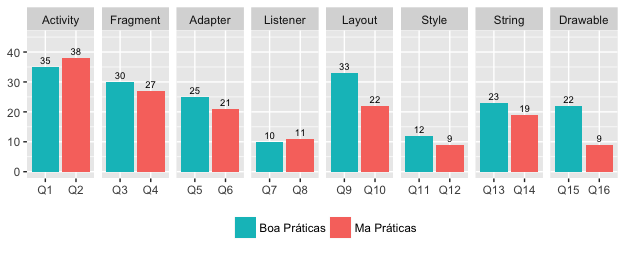
\includegraphics[width=1\linewidth]{phase1-survey-answers3.png}
\caption{Total de respostas para cada pergunta sobre boas e más práticas nos oito elementos da camada de apresentação Android.}
\label{fig:ElementsVSAnswers}
\end{figure*}

O elemento que recebeu menos respostas sobre \textbf{\small boas práticas} foi o \textit{Listener}, sendo respondida por 10 dos 45 participantes. Os elementos que receberam menos respostas sobre \textbf{\small más práticas} foram os recursos de \textit{Style} e \textit{Drawable}, sendo que ambos foram respondidos por apenas 9 dos 45 participantes. Dentre os componentes, os que receberam mais respostas foram \textit{Activities} e \textit{Fragments}, ambos sendo respondidos por pelo menos 27 participantes. Dentre os recursos, o que recebeu mais resposta foi o recurso de \textit{Layout}, sendo respondido por pelo menos 22 dos 45 participantes. De modo geral, perguntas sobre boas práticas foram mais respondidas do que as perguntas sobre más práticas, exceto sobre \textit{Activities} e \textit{Listeners}.

O processo de codificação resultou em 46 categorias, das quais consideramos para a derivação dos maus cheiros todas as que apresentaram ocorrências maior ou igual a cinco, com base no número de Nielsen \cite{NielsenMagicNumber:00}. Deste modo, 22 categorias foram consideradas. Dessas 22, desconsideramos mais 2 por se tratar de (i) um mau cheiro tradicional (Classe Grande) e (ii) um aspecto da orientação a objetos (Herança). Resultando em 20 categorias para a derivação dos maus cheiros da camada de apresentação Android. 

% A escolha do número três como número mínimo de repetições para se derivar um mau cheiro é porque evita a invariabilidade do número 1, a coincidência do número 2 e já representa alguma variação \cite{campos2001estatistica}. 

% MOVIDO PARA DISCUSSÕES
% É interessante notar que nosso processo de codificação também resultou em conclusões {\small \textbf{similares}} as de algumas pesquisas anteriores, de que aplicativos Android são fortemente afetados pelo mau cheiro tradicional \textit{Large Class} conforme citado por Verloop \cite{MobileSmells:13}, e que é pouco ou quase nada usado herança para estruturar o \textit{design} do código, conforme citado por Minelli e Lanza \cite{Mantyla2013}. Como nosso foco não estava em avaliar a presença de maus cheiro tradicionais ou práticas de orientações a objetos em aplicativos Android, não trabalhamos em cima desses resultados. 

% Cada uma das 20 categorias consideradas resultou em um mau cheiro de código Android, dos quais 9 são relacionados a componentes da camada de apresentação Android e 11 relacionados a recursos Android. A definição dos maus cheiros foram embasadas nas respostas de S$_1$, por exemplo, algumas respostas que embasaram o mau cheiro \textsc{Componente de UI Cérebro} foram ``Fazer lógica de negócio [em Activities]''\footnote{Todo texto em inglês foi traduzido livremente ao longo da dissertação} (P16). ``Colocar regra de negócio no Adapter'' (P19), ``Manter lógica de negócio em Fragments'' (P11), ``Elas [Activities] representam uma única tela e apenas interagem com a UI, qualquer lógica deve ser delegada para outra classe'' (P16) onde de P1 a P45 representam cada um dos 45 respondente. De modo a tornar a leitura dos maus cheiros mais enxuta, na Seção \ref{phase1-code-smells-catalog} apresentamos a descrições derivadas e no compilamos no Apêndice \ref{appendix:smells-purpose-of-solution} algumas respostas de exemplo que foram usadas para embasá-las.

A Tabela \ref{tab:CategoriesVSFrequency} apresenta o total de ocorrências segmentadas por elemento da camada de apresentação Android das 20 categorias consideradas para a derivação dos maus cheiros. Por exemplo, a categoria \textsc{\small Componente de UI Cérebro} apresenta 29 na coluna \textit{Activity}, 16 na coluna \textit{Fragment}, 14 na coluna \textit{Adapter} e 1 na coluna \textit{Listener}, isso significa que 29 ocorrências foram em respostas sobre boas e más práticas em \textit{Activities}, 16 ocorrências foram em respostas sobre boas e más práticas em \textit{Fragments} e assim por diante. O número sobrescrito, entre parênteses, ao lado do nome da categoria indica o total de ocorrências, ou seja, a soma das ocorrências em todos os elementos Android.

Na Figura \ref{fig:ElementsVSAnswers} o total de respostas sobre boas e más práticas em \textit{Activities} é de 73 (somatória das colunas Q1 e Q2), e na Tabela \ref{tab:CategoriesVSFrequency} o total de respostas na coluna \textit{Activity} é de 49. Essa diferença ocorre pois, na figura estamos considerando as respostas de todas as 46 categorias, enquanto na tabela estamos consideramos apenas as respostas às 20 categorias consideradas.

\begin{table}[!htb]
\centering
\renewcommand*{\arraystretch}{1}
\caption{Total de respostas sobre boas e más práticas em cada elemento da camada de apresentação Android.}
\footnotesize 
\begin{tabular}{@{}p{7cm}@{}cccccccccp{3cm}}
\toprule
\textbf{Mau Cheiro} & \rot[32][2em]{\textbf{Activity}} & \rot[32][2em]{\textbf{Fragment}} & \rot[32][2em]{\textbf{Adapter}} & \rot[32][2em]{\textbf{Listener}} & \rot[32][2em]{\textbf{Layout}} & \rot[32][2em]{\textbf{String}} & \rot[32][2em]{\textbf{Style}} & \rot[32][2em]{\textbf{Drawable}} \\ 
\toprule
\textsc{Componente de UI Cérebro}$^{(60)}$       & 29  & 16  & 14  & 1   & -    & -   & -   & -  &  \\
\textsc{Componente de UI Acoplado}$^{(18)}$      & 2   & 10  & 3   & 3   & -    & -   & -   & -  &  \\
\textsc{Comportamento Suspeito}$^{(17)}$         & 4   & -   & 3   & 10  & -    & -   & -   & -  &  \\
\textsc{Adapter Consumista}$^{(13)}$             & -   & -   & 13  & -   & -    & -   & -   & -  &  \\
\textsc{Uso Excessivo de Fragments}$^{(9)}$      & -   & 9   & -   & -   & -    & -   & -   & -  &  \\
\textsc{Componente de UI Fazendo IO}$^{(9)}$     & 5   & 3   & 1   & -   & -    & -   & -   & -  &  \\
\textsc{Não Uso de Fragment}$^{(8)}$             & 4   & 4   & -   & -   & -    & -   & -   & -  &  \\
\textsc{Ausência de Arquitetura}$^{(6)}$         & 4   & 2   & -   & -   & -    & -   & -   & -  &  \\
\textsc{Adapter Complexo}$^{(6)}$                & -   & -   & 5   & -   & 1    & -   & -   & -  &  \\
\textsc{Nome de Recurso Despadronizado}$^{(24)}$ & -   & -   & -   & -   & 5    & 10  & 5   & 3  &  \\ 
\textsc{Recurso Mágico}$^{(23)}$                 & -   & -   & -   & -   & 6    & 15  & 2   & -  &  \\ 
\textsc{Layout Profundamente Aninhado}$^{(19)}$  & -   & -   & 1   & -   & 18   & -   & -   & -  &  \\ 
\textsc{Imagem Tradicional Dispensável}$^{(18)}$ & -   & -   & -   & -   & 1    & -   & -   & 17 &  \\ 
\textsc{Layout Longo ou Repetido}$^{(14)}$       & -   & -   & -   & -   & 14   & -   & -   & -  &  \\ 
\textsc{Imagem Faltante}$^{(12)}$                & -   & -   & -   & -   & 2    & -   & -   & 10 &  \\ 
\textsc{Longo Recurso de Estilo}$^{(8)}$         & -   & -   & -   & -   & -    & -   & 8   & -  &  \\ 
\textsc{Recurso de String Bagunçado}$^{(8)}$     & -   & -   & -   & -   & -    & 8   & -   & -  &  \\ 
\textsc{Atributos de Estilo Repetidos}$^{(7)}$   & -   & -   & -   & -   & 3    & -   & 4   & -  &  \\ 
\textsc{Reúso Inadequado de String}$^{(6)}$      & -   & -   & -   & -   & -    & 6   & -   & -  &  \\ 
\textsc{Listener Escondido}$^{(5)}$              & -   & -   & -   & 5   & -    & -   & -   & -  &  \\ 
\bottomrule
\end{tabular}
\label{tab:CategoriesVSFrequency}
\end{table}

Vale observar que um mesmo mau cheiro pode afetar mais de um elemento da camada de apresentação Android. Por meio da Tabela \ref{tab:CategoriesVSFrequency}, podemos obter sugestões sobre quais elementos Android um mau cheiro afeta através do cruzamento do número de ocorrências, ou seja, se há ocorrências, possivelmente o mau cheiro respectivo afeta o elemento respectivo. Por exemplo, o mau cheiro \textsc{\small Componente de UI Cérebro} se apresenta em 4 componentes: \textit{Activities} com 29 ocorrência, \textit{Fragments} com 16, \textit{Adapters} com 14 e \textit{Listeners} com 1, e de fato, esse mau cheiro pode afetar todos esses componentes. 

Entretanto, para outros maus cheiros, essa sugestão não é verdade. Por exemplo, no caso do mau cheiro \textsc{\small Layout Profundamente Aninhado}, apesar de haver 1 ocorrência em \textit{Adapter}, esse mau cheiro não o afeta. A resposta que originou essa ocorrência indicou na verdade, uma boa prática em recursos de \textit{layout}: \textit{``Criar layouts realmente leves.''}~(P36). Esse tipo de análise da resposta foi cuidadosamente realizado para a escrita da definição textual dos maus cheiros a serem apresentados na próxima seção.


\subsubsection{Maus Cheiros Propostos}
\label{phase1-code-smells-derivation}


A Tabela \ref{tab:Smells} apresenta a lista e uma breve descrição dos 20 maus cheiros Android propostos derivados das 20 categorias com cinco ocorrências ou mais, resultante do processo de codificação. Os 9 primeiros maus cheiros afetam componentes da camada de apresentação Android, os 11 seguintes afetam recursos Android. 

As definições foram embasadas nas respostas obtidas\footnote{Todo texto em inglês foi traduzido livremente ao longo da dissertação}. Por exemplo, algumas respostas que embasaram o mau cheiro \textsc{\small Componente de UI Cérebro} foram: \textit{``Fazer lógica de negócio [em Activities]''} (P16). \textit{``Colocar regra de negócio no Adapter''} (P19), \textit{``Manter lógica de negócio em Fragments''} (P11), \textit{``Elas [Activities] representam uma única tela e apenas interagem com a UI, qualquer lógica deve ser delegada para outra classe''} (P16) onde de P1 a P45 representam cada um dos 45 respondente. Com o objetivo de tornar a leitura mais simples, as respostas usadas para embasá-los estão disponíveis no Apêndice \ref{appendix:smells-purpose-of-solution}.


Nos parágrafos seguintes apresentamos de forma textual a definição dos maus cheiros, bem como os elementos afetados por cada mau cheiro e os sintomas relacionados.

\begin{table}[h!]
\centering
\renewcommand*{\arraystretch}{1}
\caption{Lista dos 20 maus cheiros na camada de apresentação Android e breve descrição dos sintomas.}
\footnotesize 
\begin{tabular}{@{}p{6.6cm}@{}p{10cm}@{}}
\toprule
\textbf{Nome} & \textbf{Descrição} \\ 
\toprule
\textsc{Componente de UI Cérebro}$^{(60)}$            & Componentes de UI com lógicas de negócio.  \\
\textsc{Componente de UI Acoplado}$^{(18)}$           & Componentes de UI com referência concretas um para o outro.  \\
\textsc{Comportamento Suspeito}$^{(17)}$              & \textit{Listener} sendo implementado dentro de outro componente de UI.  \\
\textsc{Adapter Consumista}$^{(13)}$                  & Adapters que não usam o padrão \textit{ViewHolder}.  \\
\textsc{Uso Excessivo de Fragments}$^{(9)}$           & Uso de \textit{fragments} sem uma necessidade explícita. \\
\textsc{Componente de UI Fazendo IO}$^{(9)}$          & Componentes de UI fazendo acesso a internet ou banco de dados.  \\
\textsc{Não Uso de Fragment}$^{(8)}$                  & Não usar nenhum \textit{Fragment}.  \\
\textsc{Ausência de Arquitetura}$^{(6)}$              & Aplicativos sem uma arquitetura conhecida.  \\
\textsc{Adapter Complexo}$^{(6)}$                     & \textit{Adapters} com condicionais e \textit{loops}. \\
\textsc{Nome de Recurso Despadronizado}$^{(24)}$      & Recursos com nomes despadronizados.      \\
\textsc{Recurso Mágico}$^{(23)}$                      & Textos, números ou cores ``\textit{hardcoded}''.   \\
\textsc{Layout Profundamente Aninhado}$^{(19)}$       & Recurso de layout com mais de três níveis de \textit{Viwes} aninhadas.   \\
\textsc{Imagem Tradicional Dispensável}$^{(18)}$      & Imagens que poderiam ser transformadas em recurso gráfico.   \\
\textsc{Layout Longo ou Repetido}$^{(14)}$            & Recurso de \textit{layout} muito longo ou com trechos de código similares ou repetidos.   \\
\textsc{Imagem Faltante}$^{(12)}$                     & Imagem sem todas as resoluções padrões.   \\
\textsc{Longo Recurso de Estilo}$^{(8)}$              & Recurso de estilo único e longo.   \\
\textsc{Recurso de String Bagunçado}$^{(8)}$          & Recursos de \textit{string} sem um padrão de nomenclatura.   \\
\textsc{Atributos de Estilo Repetidos}$^{(7)}$        & Atributos de estilo repetidos em recursos de \textit{layout} ou \textit{style}.   \\
\textsc{Reúso Inadequado de String}$^{(6)}$           & \textit{Strings} sendo reutilizadas indevidamente.    \\
\textsc{Listener Escondido}$^{(5)}$                   & Atributo \textit{onClick} em recursos de \textit{layout}.  \\
\bottomrule
\end{tabular}
\label{tab:Smells}
\end{table}


% -*- root: dissertation.tex -*-
% \subsection{Catálogo de Maus Cheiros Android}
% \subsection{Catálogo de Maus Cheiros Android}
% \label{phase1-code-smells-catalog}

% Nesta seção apresentamos de forma textual a definição dos 20 maus cheiros relacionados a camada de apresentação Android, bem como os elementos afetados por cada mau cheiro e os sintomas relacionados. Ao lado do nome do mau cheiro, o número sobrescrito entre parênteses representa o total de ocorrências em respostas. 


% \subsubsection{Maus cheiros em componentes do front-end Android}
  % A Tabelas \ref{tab:Smells-Java} apresenta a lista dos maus cheiros em componentes da camada de apresentação Android, suas respectivas estrelas indicando a confiabilidade e uma breve descrição do sintoma relacionado. Em seguida, nesta seção é apresentado a descrição completa do mau cheiro.

  

  % \noindent
  % \textsc{\textbf{{\small Componente de UI Cérebro}}}$^{(12)}$ \\
  % \textbf{\small Elementos afetados:} \textit{Activities}$^{(5)}$, \textit{Fragments}$^{(3)}$, \textit{Adapters}$^{(2)}$ e \textit{Listeners}. \\
  % \textbf{\small Sintomas:} os elementos afetados podem apresentar códigos relacionados a lógica de negócio, operações de IO\footnote{Ver mau cheiro \textsc{Classes de UI Fazendo IO}.}, conversão de dados ou campos estáticos nesses elementos ao invés de apresentarem apenas códigos responsáveis por apresentar, interagir e atualizar a UI.


  % \subsubsection{\textsc{Classe de UI Inteligente (SML-J1)$^{(20)}$}}
  \noindent
  \textsc{\textbf{{\small Componente de UI Cérebro}}}$^{(60)}$ \textit{Activities}, \textit{Fragments}, \textit{Adapters} e \textit{Listeners} devem conter apenas códigos responsáveis por apresentar, interagir e atualizar a UI. São indícios do mau cheiro a existência de códigos relacionados à lógica de negócio, operações de IO\footnote{Ver mau cheiro \textsc{\small Classes de UI Fazendo IO}.}, conversão de dados ou campos estáticos nesses elementos.

      % Alguns exemplos de frases sobre \textbf{más práticas} que embasaram esse mau cheiro são: \textit{``Fazer lógica de negócio [em Activities]''}\footnote{Todo texto em inglês foi traduzido livremente ao longo da dissertação} (P16). \textit{``Colocar regra de negócio no Adapter''} (P19). \textit{``Manter lógica de negócio em Fragments''} (P11). E frases sobre \textbf{boas práticas}: \textit{``Elas [Activities] representam uma única tela e apenas interagem com a UI, qualquer lógica deve ser delegada para outra classe''} (P16). \textit{``Apenas código relacionado à Interface de Usuário nas Activities''} (P23). \textit{``Adapters devem apenas se preocupar sobre como mostrar os dados, sem trabalhá-los''} (P40). 
  
  \noindent
  \textbf{\textsc{{\small Componente de UI Acoplado}}}$^{(18)}$ \textit{Fragments}, \textit{Adapters} e \textit{Listeners}, para que possam ser reutilizados, não devem ter referência direta para quem os utiliza. São indícios do mau cheiro a existência de referência direta para \textit{Activities} ou \textit{Fragments} nesses elementos.

      % Alguns exemplos de frases sobre \textbf{más práticas} que embasaram esse mau cheiro são: \textit{``Acoplar o fragment a activity ao invés de utilizar interfaces é uma prática ruim''} (P19). \textit{``Acoplar o Fragment com a Activity''} (P10, P31 e P45). \textit{``Fragments nunca devem tentar falar uns com os outros diretamente''} (P37). \textit{``Integragir com outro Fragment diretamente''} (P45). \textit{``[Listener] conter uma referência direta à Activities''} (P4, P40). \textit{``[Adapters] alto acoplamento com a Activity''} (P10). \textit{``Acessar Activities ou Fragments diretamente''} (P45). E sobre \textbf{boa prática}: \textit{``Seja um componente de UI reutilizável. Então evite dependência de outros componentes da aplicação''} (P6).

  \noindent
  \textsc{\textbf{{\small Comportamento Suspeito}}}$^{(17)}$ \textit{Activities}, \textit{Fragments} e \textit{Adapters} não devem ser responsáveis pela implementação do comportamento dos eventos. São indícios do mau cheiro o uso de classes anônimas, classes internas ou polimorfismo (através de \textit{implements}) para implementar \textit{Listeners} de modo a responder a eventos do usuário.

      % Alguns exemplos de frases sobre \textbf{más práticas} que embasaram esse mau cheiro são: \textit{``Usar muitos anônimos pode ser complicado. Às vezes nomear coisas torna mais fácil para depuração''} (P9). \textit{``Mantenha-os [Listeners] em classes separadas (esqueça sobre classes anônimas)''} (P4). \textit{``Muitas implementações de Listener com classes anônimas''} (P8). \textit{``Declarar como classe interna da Activity ou Fragment ou outro componente que contém um ciclo de vida. Isso pode fazer com que os aplicativos causem vazamentos de memória.''} (P42). \textit{``Eu não gosto quando os desenvolvedores fazem a activity implementar o Listener porque eles [os métodos] serão expostos e qualquer um pode chamá-lo de fora da classe. Eu prefiro instanciar ou então usar ButterKnife\footnote{Biblioteca de injeção de dependência de código aberto, \url{http://jakewharton.github.io/butterknife}} para injetar cliques.''} (P44). E sobre \textbf{boas práticas}: \textit{``Prefiro declarar os listeners com implements e sobrescrever os métodos (onClick, por exemplo) do que fazer um set listener no próprio objeto''} (P32). \textit{``Tome cuidade se a Activity/Fragment é um Listener uma vez que eles são destruídos quando as configurações mudam. Isso causa vazamentos de memória.''} (P6). \textit{``Use carregamento automático de view como ButterKnife e injeção de dependência como Dagger2''} (P10).

  % \noindent
  % \textsc{\textbf{{\small Entenda o Ciclo de Vida}}}$^{(5)}$ O Ciclo de Vida de \textit{Activities}$^{(3)}$ e \textit{Fragments}$^{(3)}$ é bem delicado e elaborado, logo o uso dele exige um conhecimento mais profundo, caso contrário pode resultar em \textit{memory leaks} e outros problemas. São indícios do mau cheiro ter estes elementos como \textit{callbacks} de processos assíncronos, efetivar a transação de \textit{Fragments} (através do \textit{FragmentTransaction.commit}) após o \textit{onPause} da \textsc{Activity} ou o não tratamento da restauração do estado de \textit{Activities} e \textit{Fragments} após por exemplo, rotação da tela.

      % Alguns exemplos de frases sobre \textbf{más práticas} que embasaram esse mau cheiro são: \textit{``Não conhecer o enorme e complexo ciclo de vida de Fragment e não lidar com a restauração do estado''} (P42). \textit{``Não commitar fragmentos após o onPause e aprender o ciclo de vida se você quiser usá-los''} (P31). \textit{``Fazer Activities serem callbacks de processos assíncronos gerando memory leaks. Erros ao interpretar o ciclo de vida''} (P28). 

  \noindent
  \textsc{\textbf{{\small Adapter Consumista}}}$^{(13)}$ São indícios do mau cheiro quando \textit{Adapters} não reutilizam instâncias das \textit{views} que representam os campos a serem populados para cada item da coleção através do padrão \textit{View Holder} ou quando os mesmos possuem classes internas para reaproveitamento das \textit{views} porém não são estáticas.

      % Alguns exemplos de frases sobre \textbf{boas práticas} que embasaram esse mau cheiro são: \textit{``Reutilizar a view utilizando ViewHolder.''} (P36). \textit{``Usar o padrão ViewHolder''} (P39). P45 sugere o uso do RecyclerView, um elemento Android para a construção de listas que já implementa o padrão ViewHolder \cite{AluraViewHolder}.


  % \noindent
  % \textsc{\textbf{{\small Componente de UI Zumbi}}}$^{(2)}$ \textit{Activities} podem deixar de existir a qualquer momento, tenha cuidado ao referenciá-las. São indícios do mau cheiro a existência de referências estáticas a \textit{Activities} ou classes internas a ela ou referências não estáticas por objetos que tenham o ciclo de vida independente dela.

      % Alguns exemplos de frases sobre \textbf{más práticas} que embasaram esse mau cheiro são: \textit{``Fazer Activities serem callbacks de processos assíncronos gerando memory leaks. Erros ao interpretar o ciclo de vida''} (P28). \textit{``Ter referência estática para Activities, resultando em vazamento de memória''} (P31). E sobre \textbf{boas práticas}: \textit{``Não manter referências estáticas para Activities (ou classes anônimas criadas dentro delas)''} (P31). \textit{``Deus mata um cachorro toda vez que alguém passa o contexto da Activity para um componente que tem um ciclo de vida independente dela. Vaza memória e deixa todos tristes.''} (P4).


  \noindent
  \textsc{\textbf{{\small Uso Excessivo de Fragment}}}$^{(9)}$ \textit{Fragments} devem ser evitados. São indícios do mau cheiro quando o aplicativo não é utilizado em Tablets ou não possuem \textit{ViewPagers} e ainda assim faz o uso de \textit{Fragments} ou quando existem \textit{Fragments} no projeto que não são utilizados em mais de uma tela do aplicativo.

      % Um exemplo de frase sobre \textbf{má prática} que embasou esse mau cheiro é: \textit{``Usar muitos Fragments é uma má prática''} (P2). E frases sobre \textbf{boas práticas}: \textit{``Evite-os. Use apenas com View Pagers''} (P7). \textit{``Eu tento usar o Fragment para lidar apenas com as visualizações, como a Activity, e eu o uso apenas quando preciso deles em um layout de Tablet ou para reutilizar em outra Activity. Caso contrário, eu não uso''} (P41).


  \noindent
  \textsc{\textbf{{\small Componente de UI Fazendo IO}}}$^{(9)}$ 
      \textit{Activities}, \textit{Fragments} e \textit{Adapters} não devem ser responsáveis por operações de IO. São indícios do mau cheiro implementações de acesso a banco de dados ou internet a partir desses elementos.

      % Alguns exemplos de frases sobre \textbf{más práticas} que embasaram esse mau cheiro são: \textit{``[Activities e Fragments] fazerem requests e consultas a banco de dados''} (P26). \textit{``[Adapters] fazerem operações longas e requests de internet''} (P26). E sobre \textbf{boa prática}: \textit{``Elas [Activities] nunca devem fazer acesso a dados''} (P37).


  \noindent
  \textsc{\textbf{{\small Não Uso de Fragment}}}$^{(8)}$ \textit{Fragments} devem ser usados sempre que possível em conjunto com \textit{Activities}. É indício do mau cheiro a não existência de \textit{Fragments} na aplicação ou o uso de \textit{EditTexts}, \textit{Spinners} ou outras \textit{views} diretamente por \textit{Activities}.

      % Alguns exemplos de frases sobre \textbf{más práticas} que embasaram esse mau cheiro são: \textit{``Não usar Fragments''} (P22). \textit{``Usar todas as view (EditTexts, Spinners, etc...) dentro de Activities e não dentro de Fragments''} (P45). E sobre \textbf{boas práticas}: \textit{``Utilizar fragments sempre que possível.''} (P19), \textit{``Use um Fragment para cada tela. Uma Activity para cada aplicativo.''} (P45).         


  \noindent
  \textsc{\textbf{{\small Adapter Complexo}}}$^{(6)}$ \textit{Adapters} devem ser responsáveis por popular uma \textit{view} a partir de um único objeto, sem realizar lógicas ou tomadas de decisão. São indícios desse mau cheiro quando \textit{Adapters} contêm muitos condicionais (\textit{if} ou \textit{switch}) ou cálculos no método responsável pelo preenchimento da \textit{view}.

      % Um exemplo de frase sobre \textbf{má prática} que embasou esse mau cheiro é: \textit{``Reutilizar um mesmo adapter para várias situações diferentes, com \textit{ifs} ou \textit{switches}. Código de lógica importante ou cálculos em Adapters.''} (P23). E sobre \textbf{boa prática}: \textit{``Um Adapter deve adaptar um único tipo de item ou delegar a Adapters especializados''} (P2).



  \noindent
  \textsc{\textbf{{\small Ausência de Arquitetura}}}$^{(6)}$ São indícios do mau cheiro quando diferentes \textit{Activities} e \textit{Fragments} no projeto apresentam fluxos de código complexos, possivelmente são \textsc{\small Componente de UI Cérebro}, onde não é possível identificar uma organização padronizada entre eles que aponte para algum padrão arquitetural, como por exemplo, MVC, MVP (do inglês \textit{Model View Presenter}), MVVM (do inglês \textit{Model View ViewModel}) ou Arquitetura Limpa (do inglês \textit{Clean Architecture}).

      % Um exemplo de frase sobre \textbf{má prática} que embasou esse mau cheiro é: \textit{``Não usar um design pattern''} (P45). E frases sobre \textbf{boas práticas}: \textit{``Usar algum modelo de arquitetura para garantir apresentação desacoplada do framework (MVP, MVVM, Clean Architecture, etc)''} (P28). \textit{``Sobre MVP. Eu acho que é o melhor padrão de projeto para usar com Android''} (P45).
    
% \subsubsection{Maus cheiros em recursos Android}
%   % A Tabelas \ref{tab:Smells-Resource} apresenta a lista dos maus cheiros em recursos Android, suas respectivas estrelas indicando a confiabilidade e uma breve descrição do sintoma relacionado. Em seguida, nesta seção é apresentado a descrição completa do mau cheiro.

  \noindent
  \textbf{\textsc{{\small Nome de Recurso Despadronizado}}}$^{(24)}$
      São indícios do mau cheiro quando recursos de \textit{layout}, recursos de \textit{string}, recursos de \textit{style} e recursos \textit{drawables} não possuem um padrão de nomenclatura, seja no nome do arquivo ou dos elementos internos a eles.

      % Alguns exemplos de frases sobre \textbf{más práticas} que embasaram esse mau cheiro são: \textit{``O nome das strings sem um contexto''} (P8). \textit{``[Sobre Style Resources] Nada além de ter uma boa convenção de nomes''} (P37). \textit{``[Sobre Layout Resource] Mantenha uma convenção de nomes da sua escolha''} (P37). E sobre \textbf{boas práticas}: \textit{``Iniciar o nome de uma string com o nome da tela onde vai ser usada''} (P27). \textit{``[Sobre Layout Resource] Ter uma boa convenção de nomeação''} (P43). \textit{``[Sobre Style Resource] colocar um bom nome''} (P11). 


  \noindent
  \textbf{\textsc{{\small Recurso Mágico}}}$^{(23)}$
      Todo recurso de cor, tamanho, texto ou estilo deve ser criado em seu respectivo arquivo e então ser usado. São indícios do mau cheiro quando recursos de \textit{layout}, recursos de \textit{string} ou recursos de \textit{style} usam alguma dessas informações diretamente no código ao invés de fazer referência para um recurso existente.

      % Alguns exemplos de frases sobre \textbf{más práticas} que embasaram esse mau cheiro são: \textit{``Strings diretamente no código''} (P23). \textit{``Não extrair as strings e sobre não extrair os valores dos arquivos de layout''} (P31 e P35). E sobre \textbf{boas práticas}: \textit{``Sempre pegar valores de string ou dp de seus respectivos resources para facilitar''} (P7). \textit{``Sempre adicionar as strings em resources para traduzir em diversos idiomas''} (P36). 


  \noindent
  \textbf{\textsc{{\small Layout Profundamente Aninhado}}}$^{(19)}$
      São indícios desse mau cheiro o uso de profundos aninhamentos na construção de recursos de \textit{layout}, ou seja, \textit{ViewGroups} contendo outros \textit{ViewGroups} sucessivas vezes. O site oficial do Android conta com informações e ferramentas automatizadas para lidar com esse sintoma \cite{OptmizingViewHierarchies}. 

      % Alguns exemplos de frases sobre \textbf{más práticas} que embasaram esse mau cheiro são: \textit{``Hierarquia de views longas''} (P26). \textit{``Estruturas profundamente aninhadas''} (P4). \textit{``Hierarquias desnecessárias''} (P39). \textit{``Criar muitos ViewGroups dentro de ViewGroups''} (P45). E sobre \textbf{boas práticas}: \textit{``Tento usar o mínimo de layout aninhado''} (P4). \textit{``Utilizar o mínimo de camadas possível''} (P19). \textit{``Não fazer uma hierarquia profunda de ViewGroups''} (P8).

  \noindent
  \textbf{\textsc{{\small Imagem Tradicional Dispensável}}}$^{(18)}$
      O Android possui diversos tipos de recursos \textit{drawables} que podem substituir imagens tradicionais como \texttt{.png}, \texttt{.jpg} ou \texttt{.gif} a um custo menor em termos de tamanho do arquivo e sem a necessidade de haver versões de diferentes tamanhos/resoluções. São indícios do mau cheiro a existência de imagens com, por exemplo, cores sólidas, degradês ou estado de botões que poderiam ser substituídas por recursos \textit{drawables} de outros tipos como \textit{shapes}, \textit{state lists} ou \textit{nine-patch file}. Outro sintoma é a não existência de imagens vetoriais, que podem ser redimensionadas sem a perda de qualidade mitigando a necessidade de várias versões de um mesmo arquivo.

      % Alguns exemplos de frases sobre \textbf{más práticas} que embasaram esse mau cheiro são: \textit{``Uso de formatos não otimizados, uso de drawables onde recursos padrão do Android seriam preferíveis''} (P23). \textit{``Usar jpg ou png para formas simples é ruim, apenas as desenhe [através de Drawable Resources]''} (P37). E sobre \textbf{boas práticas}: \textit{``Quando possível, criar resources através de xml''} (P36). \textit{``Utilizar o máximo de Vector Drawables que for possível''} (P28). \textit{``Evite muitas imagens, use imagens vetoriais sempre que possível''} (P40).

  \noindent
  \textbf{\textsc{{\small Layout Longo ou Repetido}}}$^{(14)}$
      Sempre que possível, reutilizar trechos de \textit{layout}. São indícios do mau cheiro quando um recurso de \textit{layout} é muito grande ou possui trechos de código muito semelhantes ou iguais dentro dele ou a outras telas. 

      % Um exemplo de frase sobre \textbf{má prática} que embasou esse mau cheiro é: \textit{``Copiar e colar layouts parecidos sem usar includes''} (P41). \textit{``Colocar muitos recursos no mesmo arquivo de layout.''} (P23). E sobre \textbf{boas práticas}: \textit{``Sempre quando posso, estou utilizando includes para algum pedaço de layout semelhante''} (P32). \textit{``Criar layouts que possam ser reutilizados em diversas partes''} (P36). \textit{``Separe um grande layout usando include ou merge''} (P42) 

  \noindent
  \textbf{\textsc{{\small Imagem Faltante}}}$^{(12)}$
      As imagens devem ser disponibilizadas em mais de um tamanho ou resolução para que o Android possa realizar otimizações. São indícios do mau cheiro haver apenas uma versão de algum recurso \textit{drawable} do tipo \texttt{.png}, \texttt{.jpg} ou \texttt{.gif}, ou ainda, ter imagens em diretórios incorretos em termos de \textit{dpi}.

      % Alguns exemplos de frases sobre \textbf{más práticas} que embasaram esse mau cheiro são: \textit{``Ter apenas uma imagem para multiplas densidades''} (P31). \textit{``Baixar uma imagem muito grande quando não é necessário. Há melhores formas de usar memória''} (P4). \textit{``Não criar imagens para todas as resoluções''} (P44).E sobre \textbf{boas prática}: \textit{``Nada especial, apenas mantê-las em seus respectivos diretórios e ter variados tamanhos delas''} (P34). \textit{``Criar as pastas para diversas resoluções e colocar as imagens corretas''} (P36). 

  \noindent
  \textbf{\textsc{{\small Longo Recurso de Estilo}}}$^{(8)}$
      É indício do mau cheiro haver apenas um recurso de \textit{style} ou conter recursos de \textit{style} muito longos.

      % Alguns exemplos de frases sobre \textbf{más práticas} que embasaram esse mau cheiro são: \textit{``Deixar tudo no mesmo arquivo styles.xml''} (P28). \textit{``Arquivos de estilos grandes''} (P8). E sobre \textbf{boas práticas}: \textit{``Se possível, separar mais além do arquivo styles.xml padrão, já que é possível declarar múltiplos arquivos XML de estilo para a mesma configuração''} (P28). \textit{``Divida-os. Temas e estilos é uma escolha racional''} (P40).

  \noindent
  \textbf{\textsc{{\small Recurso de String Bagunçado}}}$^{(8)}$
      É indício do mau cheiro o uso de apenas um arquivo para todos os recursos de \textit{string} do aplicativo e a não existência de um padrão de nomenclatura e separação para os recursos de \textit{string} de uma mesma tela. 

      % Alguns exemplos de frases sobre \textbf{más práticas} que embasaram esse mau cheiro são: \textit{``Usar o mesmo arquivo strings.xml para tudo''} (P28). \textit{``Não orgaizar as strings quando o strings.xml começa a ficar grande''} (P42). E sobre \textbf{boas práticas}: \textit{``Separar strings por tela em arquivos XML separados. Extremamente útil para identificar quais strings pertencentes a quais telas em projetos grandes''} (P28). \textit{``Sempre busco separar em blocos, cada bloco representa uma Activity e nunca aproveito uma String pra outra tela''} (P32).

  \noindent
  \textbf{\textsc{{\small Atributos de Estilo Repetidos}}}$^{(7)}$
      É indício do mau cheiro haver recursos de \textit{layout} ou recursos de \textit{style} com blocos de atributos de estilo repetidos. 
      % , onde poderiam ser extraídos para um novo estilo e substituir o bloco de atributos repetidos pelo estilo criado.

      % Um exemplo de frase sobre \textbf{má prática} que embasou esse mau cheiro é: \textit{``Utilizar muitas propriedades em um único componente. Se tiver que usar muitas, prefiro colocar no arquivo de styles.''} (P32). E sobre \textbf{boa prática}: \textit{``Sempre que eu noto que tenho mais de um recurso usando o mesmo estilo, eu tento movê-lo para o meu style resource.''} (P34).

  \noindent
  \textbf{\textsc{{\small Reúso Inadequado de String}}}$^{(6)}$
      Cada tela deve ter seu conjunto de recursos de \textit{string}. É indício do mau cheiro reutilizar o mesmo recurso de \textit{string} em diferentes telas do aplicativo apenas porque o texto coincide.

      % Alguns exemplos de frases sobre \textbf{más práticas} que embasaram esse mau cheiro são: \textit{``Utilizar uma String pra mais de uma activity, pois se em algum momento, surja a necessidade de trocar em uma, vai afetar outra.''} (P32). \textit{``Reutilizar a string em várias telas''} (P6) \textit{``Reutilizar a string apenas porque o texto coincide, tenha cuidado com a semântica''} (P40). E sobre \textbf{boas práticas}: \textit{``Sempre busco separar em blocos, cada bloco representa uma activity e nunca aproveito uma String pra outra tela.''} (P32). \textit{``Não tenha medo de repetir strings''} (P9). 

  \noindent
  \textbf{\textsc{{\small Listener Escondido}}}$^{(5)}$
      recursos de \textit{layout} devem ser responsáveis apenas por apresentar informações. É indício do mau cheiro o uso de atributos de eventos, como o \textit{onClick}, diretamente em recursos de \textit{layout} para configurar o \textit{Listener} que responderá ao evento. \\

      % Alguns exemplos de frases sobre \textbf{más práticas} que embasaram esse mau cheiro são: \textit{``Nunca crie um listener dentro do XML. Isso esconde o listener de outros desenvolvedores e pode causar problemas até que ele seja encontrado''} (P34, P39 e P41). E sobre \textbf{boa prática}: \textit{``XML de layout deve lidar apenas com a view e não com ações''} (P41).


\begin{square}
  \small
  Nossos resultados mostram que existem maus cheiros específicos a elementos da camada de apresentação Android (QP$_1$).
\end{square}












\subsection{QP$_2$ Importância e Frequência dos Maus Cheiros Android}
\label{phase2-results}

% Participaram desta etapa da pesquisa 201 desenvolvedores de 3 continentes e 14 países diferentes. Brasileiros representam 78\%, e vieram de 18 estados diferentes. Deste modo, apesar da abrangência geográfica, entendemos que os resultados expressam majoritariamente a percepção de desenvolvedores brasileiros. 15\% dos participantes possuem uma ou mais pós-graduações e 61\% são graduados. 57\% possuem de 20 a 35 anos. 

Nossos resultados mostraram que os 20 maus cheiros propostos são considerados, em diferentes níveis, importantes e se apresentam com diferentes frequências no dia a dia do desenvolvimento Android. As distribuições relativas de frequência e importância, sobre cada afirmação apresentada no questionário, pode ser conferida nos Apêndices \ref{appendix-phase2-frequence-table} (afirmações de frequência) e \ref{appendix-phase2-importance-table} (afirmações de importância).

% Para os maus cheiros que foram apresentadas no questionário mais de uma afirmação de importância ou frequência, se mostraram com distribuição relativa muito semelhantes, variando de 6\% a no máximo 10\% de uma afirmação a outra.

\subsubsection{Resultados Gerais}
\label{phase2-general-results} 

Para análise dos maus cheiros extraímos dados estatísticos de moda (MO), mediana (ME) e desvio padrão (DP) de importância e frequência para cada um dos maus cheiros propostos. Utilizamos a MO como um classificador do mau cheiro, ou seja, se ele recebeu majoritariamente a resposta ``importante'', o classificamos como importante. Estes dados são apresentados na Tabela \ref{tab:SmellFrequencyImportance} onde podemos observar que todos os maus cheiros apresentam MO de importância maior ou igual a 3, ou seja, de ``razoavelmente importante'' a ``muito importante''. Em contrapartida, com relação à frequência, três maus cheiros (\textsc{\small Adapter Consumista}, \textsc{\small Listener Escondido} e \textsc{\small Não Uso de Fragment}) apresentaram MO igual a 2, ``raramente'', todos os demais apresentaram MO maior ou igual a 3, ou seja, de ``às vezes'' até ``muito frequente''. 

\begin{table}[!htb]
\centering
\renewcommand*{\arraystretch}{1}
\footnotesize 
\caption{Mediana (ME), moda (MO) e desvio padrão (DP) sobre a percepção da importância dos maus cheiros relacionados a componentes da camada de apresentação Android.}
\begin{tabular}{@{}p{9cm}cccp{.5cm}ccc@{}}
\toprule
\multirow{2}{*}{\textbf{Mau Cheiro}} & \multicolumn{3}{c}{\textbf{Importância}} & & \multicolumn{3}{c}{\textbf{Frequência}} \\ \cmidrule{2-4} \cmidrule{6-8}
                                      & \textbf{ME} & \textbf{MO} & \textbf{DP} & & \textbf{ME} & \textbf{MO} & \textbf{DP} \\
\bottomrule
\textsc{Componente de UI Cérebro} & 5 & 5 & 1,05 & & 3 & 4 & 1,19 \\ 
\textsc{Recurso Mágico} & 4 & 5 & 1,00 & & 3 & 4 & 1,24 \\ 
\textsc{Imagem Tradicional Dispensável} & 4 & 5 & 0,95 & & 3 & 4 & 1,23 \\ 
\textsc{Layout Longo ou Repetido} & 4 & 5 & 0,95 & & 4 & 4 & 1,07 \\ 
\textsc{Imagem Faltante} & 5 & 5 & 0,95 & & 3 & 4 & 1,25 \\ 
\textsc{Componente de UI Acoplado} & 4 & 5 & 1,02 & & 3 & 3 & 1,15 \\ 
\textsc{Classes de UI Fazendo IO} & 5 & 5 & 1,03 & & 3 & 3 & 1,29 \\ 
% \textsc{Componente de UI Zumbi} & 5 & 5 & 0,88 & & 3 & 3 & 1,16 \\ 
\textsc{Ausência de Arquitetura} & 5 & 5 & 0,82 & & 3 & 3 & 1,30 \\ 
\textsc{Adapter Complexo} & 4 & 5 & 0,91 & & 3 & 3 & 1,15 \\ 
\textsc{Nome de Recurso Despadronizado} & 5 & 5 & 0,88 & & 3 & 3 & 1,24 \\ 
\textsc{Adapter Consumista} & 5 & 5 & 0,93 & & 2 & 2 & 1,20 \\ 
\textsc{Listener Escondido} & 4 & 5 & 1,23 & & 2 & 2 & 1,29 \\ 
\textsc{Longo Recurso de Estilo} & 4 & 4 & 1,06 & & 4 & 5 & 1,18 \\ 
\textsc{Recurso de String Bagunçado} & 3 & 4 & 1,22 & & 4 & 5 & 1,18 \\ 
\textsc{Comportamento Suspeito} & 3 & 4 & 1,19 & & 3 & 4 & 1,19 \\ 
\textsc{Layout Profundamente Aninhado} & 4 & 4 & 1,12 & & 4 & 4 & 1,06 \\ 
\textsc{Atributos de Estilo Repetidos} & 4 & 4 & 0,86 & & 4 & 4 & 1,11 \\ 
\textsc{Não Uso de Fragment} & 3 & 4 & 1,34 & & 3 & 2 & 1,21 \\ 
\textsc{Reúso Inadequado de String} & 3 & 3 & 1,29 & & 4 & 4 & 1,12 \\ 
\textsc{Uso Excessivo de Fragment} & 3 & 3 & 1,36 & & 3 & 3 & 1,17 \\  
\toprule
DP Médio &  &  & 1.05 &  & &  & 1.19 \\ 
% \toprule
% \multicolumn{8}{@{}l@{}}{DP = Desvio Padrão, MO = Moda, ME = Média.} \\
\bottomrule
\end{tabular}
\label{tab:SmellFrequencyImportance}
\end{table}


Entendemos este resultado de forma positiva pois, apesar de alguns sintomas não serem tão frequentes, ainda assim são considerados com algum nível de importância de se mitigar, reforçando também a relevância desta pesquisa pois damos os primeiros passos no sentido da automatização da identificação desses maus cheiros. Com base no DP, podemos observar que, de modo geral, existe uma concordância maior sobre a importância dos maus cheiros do que sobre a frequência, pois a média do DP de importância é de 1,05, ligeiramente menor que a média do DP de frequência, que é de 1,19. 

Quanto menor o DP maior a concordância entre os participantes sobre determinado mau cheiro. Podemos observar que os maus cheiros que tiveram maior concordância com relação à sua importância foram: \textsc{\small Adapter Complexo}, \textsc{\small Adapter Consumista}, \textsc{\small Atributos de Estilo Repetidos}, \textsc{\small Ausência de Arquitetura}, \textsc{\small Imagem Faltante}, \textsc{\small Imagem Tradicional Dispensável}, \textsc{\small Layout Longo ou Repetido}, \textsc{\small Nome de Recurso Despadronizado}, todos com DP menor que 1. Sobre a concordância relacionada à frequência, nenhum dos maus cheiros obteve DP menor que 1, mas os mais próximos, indicando maior concordância sobre sua frequência são: \textsc{\small Layout Profundamente Aninhado} com DP de 1,06 e \textsc{\small Longo Recurso de Estilo} com DP 1,07. 


\subsubsection{Importância dos Maus Cheiros}

Para análise dos dados, simplificamos a escala \textit{likert} de importância de modo que, os maus cheiros de MO 3, ``razoavelmente importante'', são classificados como sendo de \textbf{\small importância moderada}, os maus cheiros de MO 4 ou 5, respectivamente ``importante'' e ``muito importante'', são classificados de \textbf{\small importância alta}. Nenhum mau cheiro teve MO 1 ou 2, respectivamente ``não é importante'' e ``pouco importante'', logo, não criamos classificações para essas opções. 

A Tabela \ref{tab:SmellImportance} apresenta a lista dos maus cheiros de acordo com seu nível de importância, alta ou moderada. Podemos observar que as duas primeiras colunas contém os 18 maus cheiros classificados com \textbf{\small importância alta}. Dentre eles, a maioria dos maus cheiros (10) afetam recursos Android: \textsc{\small Longo Recurso de Estilo}, \textsc{\small Layout Profundamente Aninhado}, \textsc{\small Atributos de Estilo Repetidos}, \textsc{\small Nome de Recurso Despadronizado}, \textsc{\small Recurso Mágico}, \textsc{\small Imagem Faltante}, \textsc{\small Imagem Tradicional Dispensável}, \textsc{\small Layout Longo ou Repetido}, \textsc{\small Recurso de String Bagunçado} e \textsc{\small Listener Escondido}.

\begin{table}[!htb]
\centering
\renewcommand*{\arraystretch}{1}
\footnotesize 
\caption{Listagem dos maus cheiros da camada de apresentação Android de acordo com seu nível de importância, alta ou moderada.}
\begin{tabular}{@{}p{5.2cm}p{5.2cm}p{5.2cm}@{}}
\toprule
\multicolumn{2}{c}{\textbf{Importância Alta}} & \multicolumn{1}{c}{\textbf{Importância Moderada}}  \\ 
\bottomrule
\textsc{\scriptsize Adapter Complexo}              & \textsc{\scriptsize Atributos de Estilo Repetidos} & \textsc{\scriptsize Reúso Inadequado de String} \\ 
\textsc{\scriptsize Adapter Consumista}            & \textsc{\scriptsize Comportamento Suspeito}        & \textsc{\scriptsize Uso Excessivo de Fragment} \\ 
\textsc{\scriptsize Ausência de Arquitetura}       & \textsc{\scriptsize Layout Profundamente Aninhado} \\ 
\textsc{\scriptsize Classes de UI Fazendo IO}      & \textsc{\scriptsize Longo Recurso de Estilo}       \\ 
\textsc{\scriptsize Componente de UI Acoplado}     & \textsc{\scriptsize Não Uso de Fragment}           \\ 
\textsc{\scriptsize Componente de UI Cérebro}      & \textsc{\scriptsize Recurso de String Bagunçado}   \\ 
\textsc{\scriptsize Recurso Mágico}                & \textsc{\scriptsize Imagem Faltante}               \\ 
\textsc{\scriptsize Imagem Tradicional Dispensável}& \textsc{\scriptsize Layout Longo ou Repetido}      \\ 
\textsc{\scriptsize Listener Escondido}            & \textsc{\scriptsize Nome de Recurso Despadronizado}\\ 
\toprule
\multicolumn{2}{c}{18} & \multicolumn{1}{c}{2}  \\ 
\bottomrule
\end{tabular}
\label{tab:SmellImportance}
\end{table}

Enquanto que 8 dos maus cheiros de \textbf{\small importância alta} afetam componentes da camada de apresentação Android: \textsc{\small Adapter Complexo}, \textsc{\small Adapter Consumista}, \textsc{\small Ausência de Arquitetura}, \textsc{\small Classes de UI Fazendo IO}, \textsc{\small Componente de UI Cérebro}, \textsc{\small Atributos de Estilo Repetidos}, \textsc{\small Comportamento Suspeito} e \textsc{\small Não Uso de Fragment}. Apenas 2 maus cheiros: \textsc{\small Reúso Inadequado de String} e \textsc{\small Uso Excessivo de Fragment}, listados na última coluna da tabela, são de \textbf{\small importância moderada}, sendo 1 relacionado a recursos e outro componentes da camada de apresentação Android. 

A Figura \ref{fig:phase2-results-importance} apresenta a distribuição relativa de importância dos maus cheiros. Apresentamos negativo (em vermelho) o percentual relacionado às respostas ``não é importante''. 

\begin{figure*}[!htb]
  \centering
  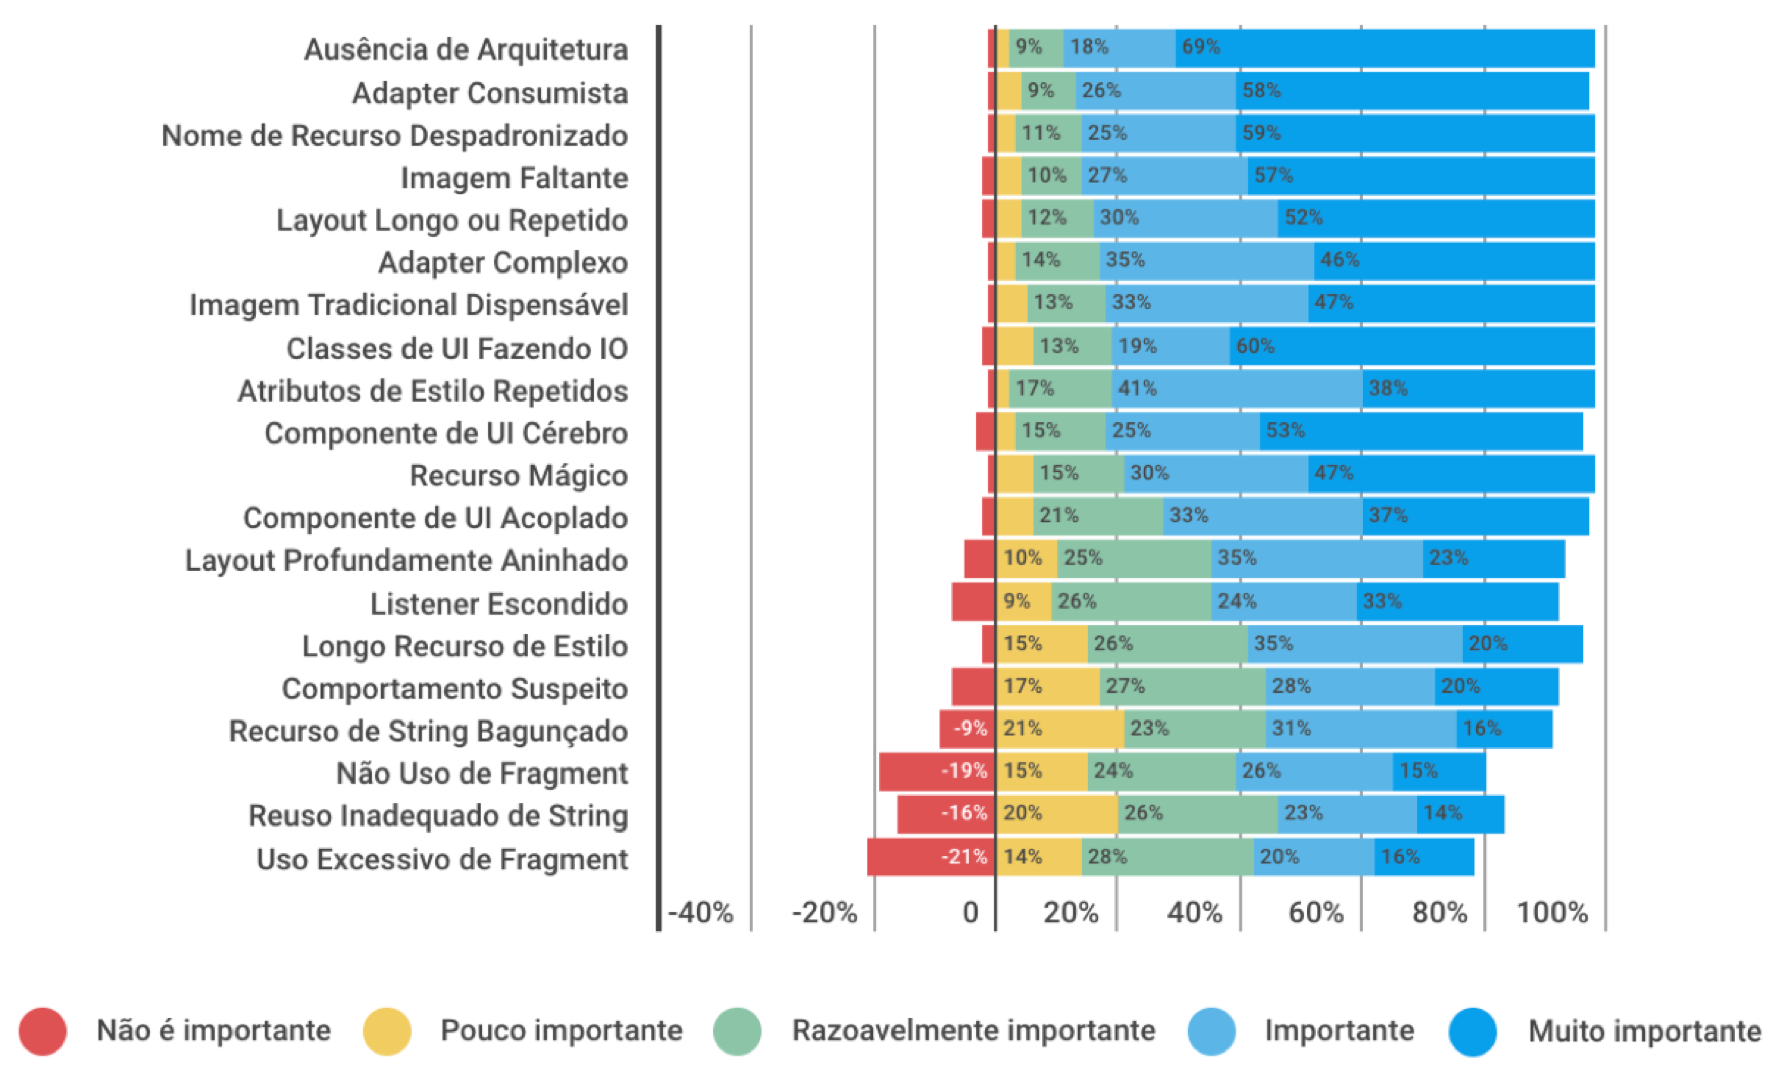
\includegraphics[width=1\textwidth]{phase2-results-importance2.png}
  \caption{Distribuição relativa de importância dos maus cheiros propostos.}
  \label{fig:phase2-results-importance}
  % \vspace{-.5cm} 
\end{figure*}

Os três maus cheiros considerados menos importantes foram \textsc{\small Reúso Inadequado de String}, \textsc{\small Não Uso de Fragment} e \textsc{\small Uso Excessivo de Fragment}, com mais de 16\% dos participantes indicando ``não é importante'', menos de 26\% indicando ``importante'' e menos de 16\% indicando ``muito importante''. São os mesmos que tiveram menor concordância com relação à sua importância, todos com DP acima de 1,28. Esses dados sugerem que desenvolvedores Android ainda têm dúvidas sobre o impacto negativo desses maus cheiros no código.


\subsubsection{Frequência dos Maus Cheiros}

Para análise dos dados, simplificamos a escala \textit{likert} de frequência de modo similar ao de importância, onde maus cheiros de MO 2, ``raramente'', são classificados como \textbf{\small frequência baixa}, os maus cheiros de MO 3, ``às vezes'', são classificados como \textbf{\small frequência moderada} e os maus cheiros de MO 4 ou 5, respectivamente ``frequente'' e ``muito frequente'', são classificados de \textbf{\small frequência alta}. Nenhum mau cheiro teve MO 1, ``nunca'', e portanto não criamos classificação para essa opção. A Tabela \ref{tab:SmellFrequency} apresenta a lista dos maus cheiros de acordo com seu nível de frequência, alta, moderada ou baixa. 

\begin{table}[!htb]
\centering
\renewcommand*{\arraystretch}{1}
\footnotesize 
\caption{Listagem dos maus cheiros da camada de apresentação Android de acordo com seu nível de frequência, alta, moderada ou baixa.}
\begin{tabular}{@{}p{5.2cm}p{5.2cm}p{5.2cm}@{}}
\toprule
\multicolumn{1}{c}{\textbf{Frequência Alta}} & \multicolumn{1}{c}{\textbf{Frequência Moderada}} & \multicolumn{1}{c}{\textbf{Frequência Baixa}} \\ 
\bottomrule
\textsc{\scriptsize Atributos de Estilo Repetidos}  & \textsc{\scriptsize Adapter Complexo}               & \textsc{\scriptsize Adapter Consumista} \\ 
\textsc{\scriptsize Componente de UI Cérebro}       & \textsc{\scriptsize Ausência de Arquitetura}        & \textsc{\scriptsize Listener Escondido} \\ 
\textsc{\scriptsize Imagem Faltante}                & \textsc{\scriptsize Classes de UI Fazendo IO}       & \textsc{\scriptsize Não Uso de Fragment} \\ 
\textsc{\scriptsize Imagem Tradicional Dispensável} & \textsc{\scriptsize Componente de UI Acoplado}      \\ 
\textsc{\scriptsize Layout Longo ou Repetido}       & \textsc{\scriptsize Uso Excessivo de Fragment}      \\ 
\textsc{\scriptsize Layout Profundamente Aninhado}  & \textsc{\scriptsize Comportamento Suspeito}         \\ 
\textsc{\scriptsize Longo Recurso de Estilo}        & \textsc{\scriptsize Nome de Recurso Despadronizado} \\ 
\textsc{\scriptsize Recurso Mágico}                 \\ 
\textsc{\scriptsize Reúso Inadequado de String}     \\ 
\textsc{\scriptsize Recurso de String Bagunçado}    \\ 
\toprule
\multicolumn{1}{c}{10} & \multicolumn{1}{c}{7} & \multicolumn{1}{c}{3}\\ 
\bottomrule
\end{tabular}
\label{tab:SmellFrequency}
\end{table}

É interessante notar que, maus cheiros em recursos são percebidos mais frequentemente que os maus cheiros em componentes da camada de apresentação Android. Podemos observar na Tabela \ref{tab:SmellFrequency} que, 9 dentre os 10 maus cheiros de \textbf{\small frequência alta} são em recursos Android: \textsc{\small Atributos de Estilo Repetidos}, \textsc{\small Imagem Faltante}, \textsc{\small Imagem Tradicional Dispensável}, \textsc{\small Layout Longo ou Repetido}, \textsc{\small Layout Profundamente Aninhado}, \textsc{\small Longo Recurso de Estilo}, \textsc{\small Recurso Mágico}, \textsc{\small Reúso Inadequado de String} e \textsc{\small Recurso de String Bagunçado}. Enquanto que apenas o mau cheiro de \textbf{\small frequência alta}, \textsc{\small Componente de UI Cérebro}, é relacionado a componentes da camada de apresentação Android.

Nos demais níveis de frequência, essa situação se inverte, sendo os maus cheiros em componentes da camada de apresentação Android, maioria. Dentre os maus cheiros de \textbf{\small frequência moderada}, 6 dentre os 7 são relacionados a componentes: \textsc{\small Adapter Complexo}, \textsc{\small Ausência de Arquitetura}, \textsc{\small Classes de UI Fazendo IO}, \textsc{\small Componente de UI Acoplado}, \textsc{\small Uso Excessivo de Fragment} e \textsc{\small Comportamento Suspeito}. Apenas o mau cheiro \textsc{\small Nome de Recurso Despadronizado} é relacionado a recursos Android. Dentre os maus cheiro de \textbf{\small frequência baixa}, 2 dentre os 3 são relacionados a componentes da camada de apresentação Android: \textsc{\small Adapter Consumista} e \textsc{\small Não Uso de Fragment}. E apenas o mau cheiro \textsc{\small Listener Escondido} é relacionado a recursos Android.

\begin{figure*}[!htb]
  \centering
  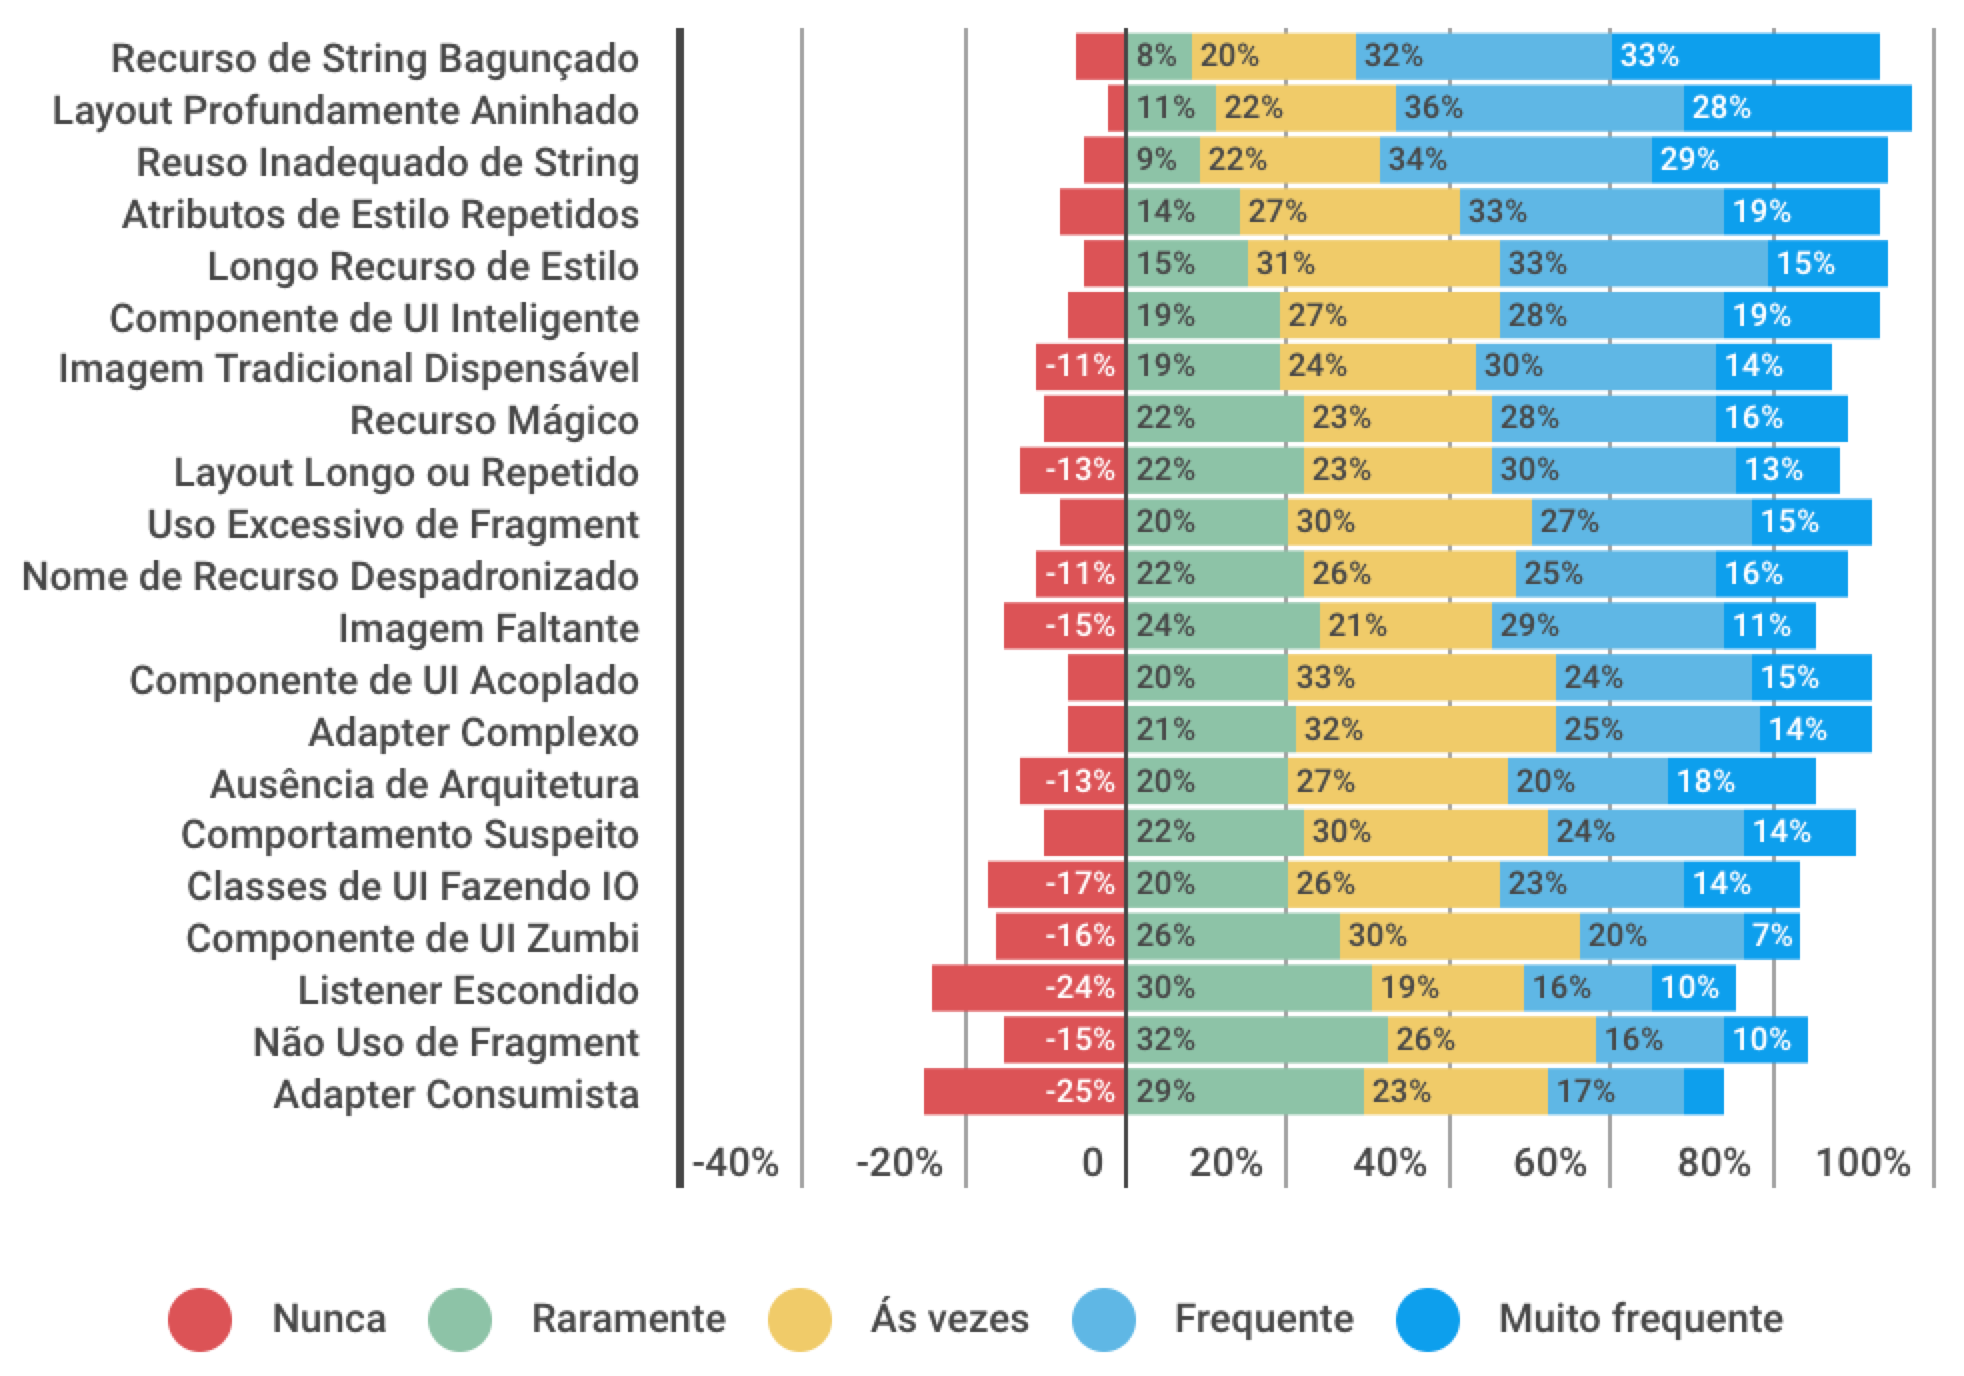
\includegraphics[width=1\textwidth]{phase2-results-frequence.png}
  \caption{Distribuição relativa de frequência dos maus cheiros propostos.}
  \label{fig:phase2-survey-frequence}
  % \vspace{-.5cm} 
\end{figure*}

A Figura \ref{fig:phase2-survey-frequence} apresenta a distribuição relativa de frequência dos maus cheiros. Apresentamos negativo (em vermelho) o percentual relacionado às respostas ``nunca''. Os maus cheiros menos percebidos (com mais de 20\% de respostas ``nunca'') foram \textsc{\small Adapter Consumista} (25\%) e \textsc{\small Listener Escondido} (24\%). Todos os demais maus cheiros são percebidos no dia a dia, com frequência moderada ou alta, por pelo menos 75\% dos participantes.

\textsc{\small Adapter Consumista} foi o mau cheiro menos percebido no dia a dia por desenvolvedores Android (25\% dos participantes indicaram ``nunca''). Entretanto ele é o segundo considerado mais importante (58\% dos participantes indicaram ``muito importante'' e 26\% indicaram ``importante''). Esses dados sugerem que desenvolvedores já estão cientes dos benefícios do uso do padrão \textit{ViewHolder} \cite{AluraViewHolder} e encontraram formas de mitigar este mau cheiro. Na seção \ref{sec:discussoes} realizamos uma breve discussão sobre esse resultado. 

\textsc{\small Listener Escondido} foi o segundo mau cheiro menos percebido no dia a dia por desenvolvedores Android (24\% dos participantes indicaram ``nunca''). Entretanto se apresenta dentre os maus cheiros considerados mais importantes (33\% dos participantes indicaram ``muito importante'' e 24\% indicaram ``importante''). Esses dados sugerem que os desenvolvedores consideram importante evitar o uso do atributo \textit{onClick} em XMLs de \textit{layout} e aparentemente, muitos desenvolvedores já estão cientes disso no dia a dia, uma vez que ele se apresenta dentre os 6 menos percebidos. \\


\begin{square}
  \small
  Nossos resultados mostram que os maus cheiros propostos são considerados importantes e frequentes no dia a dia do desenvolvimento Android (QP$_2$). 
\end{square}




% -*- root: dissertation.tex -*-
\subsection{QP$_3$ Percepção dos Desenvolvedores sobre os Maus Cheiros Android}
\label{phase3-results}

Nossos resultados mostram que códigos afetados por 6 dos 7 maus cheiros avaliados são percebidos como códigos problemáticos por desenvolvedores Android, são eles: \textsc{\small Componente de UI Cérebro}, \textsc{\small Componente de UI Acoplado}, \textsc{\small Comportamento Suspeito}, \textsc{\small Adapter Complexo}, \textsc{\small Layout Profundamente Aninhado} e \textsc{\small Atributos de Estilo Repetidos}. Não foi possível concluir a percepção sobre o mau cheiro \textsc{\small Longo Recurso de Estilo} pois a média de 30 pontos não foi suficiente para chegarmos a uma conclusão, sendo necessário coletar mais dados. A seguir apresentamos detalhes das percepções dos desenvolvedores sobre os maus cheiros avaliados.

% Com o objetivo de aumentar a confiabilidade do experimento, nosso objetivo foi obter em média 30 pontos de observação para cada mau cheiro avaliado. Para 6 maus cheiros essa quantidade de pontos foi suficiente, porém para o mau cheiro \textsc{\small Longo Recurso de Estilo} não, 


\subsubsection{Resultados}
\label{sec:results-phase3}

Na Figura \ref{fig:components-violins}, apresentamos os gráficos violino que consolidam a percepção de desenvolvedores sobre os 4 maus cheiros relacionados a componentes da camada de apresentação Android (\textsc{\small Componente de UI Cérebro}, \textsc{\small Componente de UI Acoplado}, \textsc{\small Comportamento Suspeito} e \textsc{\small Adapter Complexo}) contra componentes Android limpos. De modo similar, na Figura \ref{fig:resources-violins}, apresentamos os gráficos violino que consolidam a percepção de desenvolvedores sobre os 3 maus cheiros relacionados à recursos Android (\textsc{\small Layout Profundamente Aninhado}, \textsc{\small Atributos de Estilo Repetidos} e \textsc{\small Longo Recurso de Estilo}) contra recursos limpos. 

\begin{figure*}[!htb]
\centering
\imagewidth=0.54\textwidth
\captionsetup[subfigure]{width=.9\imagewidth,justification=raggedright}%
\begin{subfigure}[t]{.49\textwidth}
  \centering
  \hspace*{-1cm}%
  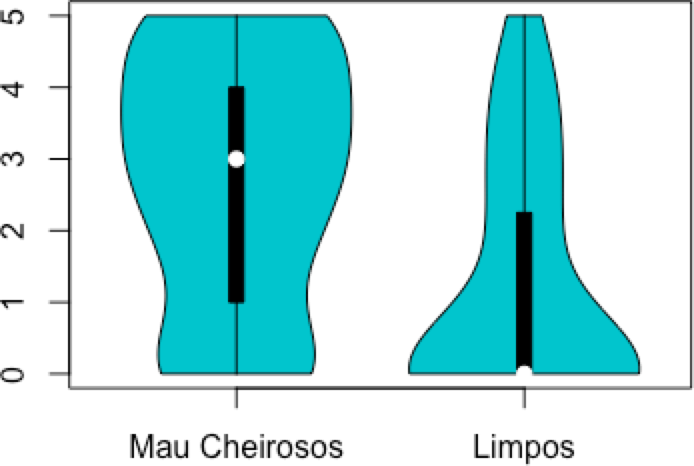
\includegraphics[width=.8\textwidth]{phase3-components-clean-smelly-violins-cutted.png}
  \caption{Componentes.}
  \label{fig:components-violins}
\end{subfigure}
\begin{subfigure}[t]{.49\textwidth}
  \centering
  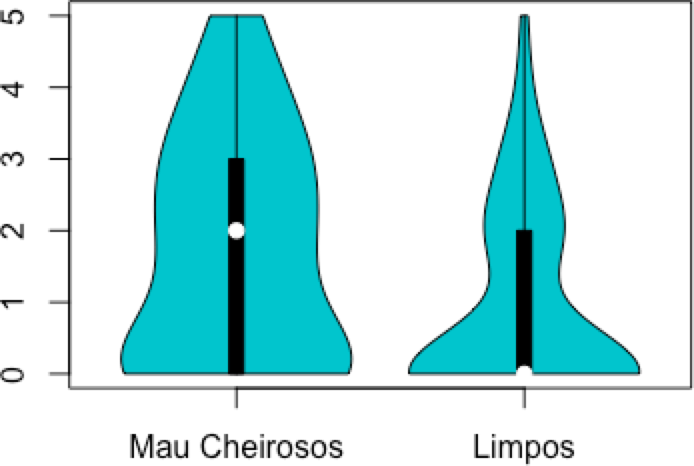
\includegraphics[width=.8\textwidth]{phase3-resources-clean-smelly-violins-cutted.png}
  \caption{Recursos.}
  \label{fig:resources-violins}
\end{subfigure}% 
\caption{Análise de severidade em componentes e recursos mau cheirosos e limpos.}
\label{fig:smelly-clean-consolidado}
% \vspace{-.5cm} 
\end{figure*}

No eixo y, 0 (zero) indica os códigos não percebidos pelos desenvolvedores como problemáticos (ou seja, responderam ``não'' à questão: ``\emph{Esta classe exibe algum problema de design e/ou implementação?}''), enquanto que os valores de 1 a 5 indicam o nível de severidade para o problema percebido pelo desenvolvedor. No eixo x, os gráficos são autoexplicativos. Nos parágrafos seguintes explicamos os dados de cada gráfico de modo que, as medianas são indicadas pela bolinha branca e o 3º quartil (Q3) é representado pela linha preta mais grossa na vertical.

Podemos observar na Figura \ref{fig:components-violins} que componentes afetados pelos maus cheiros Android tiveram mediana de severidade igual a 3 (Q3 = 4). Isso indica que, como esperado, desenvolvedores percebem códigos afetados pelos maus cheiros em componentes da camada de apresentação Android como problemáticos. Como comparação, componentes Android limpos tiveram mediana de severidade igual a 0 (Q3 = 2). A diferença na percepção dos desenvolvedores entre componentes Android mau cheirosos e componentes limpos é estatisticamente significante ($\alpha$ = 1,18e-06) com médio tamanho de efeito (\textit{d} = 0,46). 

Na Figura \ref{fig:resources-violins}, podemos observar que recursos afetados pelos maus cheiros Android tiveram mediana de severidade é igual a 2 (Q3 = 3). Isso mostra que, recursos afetados pelos maus cheiros Android são percebidos como problemáticos, ainda que menos que os maus cheiros em componentes Android. Como comparação, recursos Android limpos tiveram mediana de severidade igual a 0 (Q3 = 2). A diferença na percepção dos desenvolvedores entre os recursos mau cheirosos e recursos limpos também é estatisticamente significante ($\alpha$ = 1,24e-03) com pequeno tamanho de efeito (\textit{d} = 0,29).

 % - bem como de componentes e recursos de \textit{Style} e \textit{Layout} limpos - Figura \ref{fig:clean-violins}.   
Além disso, relatamos a percepção dos desenvolvedores sobre cada mau cheiro Android individualmente na Figura \ref{fig:smellys-violins}. O mau cheiro \textsc{\small Componente de UI Acoplado} (CA) é o mais percebido pelos desenvolvedores e com maior gravidade, apresenta mediana de severidade igual a 4 (Q3 = 5). Em seguida temos os maus cheiros \textsc{\small Componente de UI Cérebro} (CC), \textsc{\small Adapter Complexo} (AC) e \textsc{\small Comportamento Suspeito} (CS) todos com mediana de severidade igual a 3. Isso indica que, como esperado, são percebidos pelos desenvolvedores como sendo seriamente problemáticos. Podemos notar que, de modo geral, recursos afetados pelos maus cheiros Android -- \textsc{\small Longo Recurso de Estilo} (LE), \textsc{\small Layout Profundamente Aninhado} (LA) e \textsc{\small Atributos de Estilo Repetidos} (AR) -- foram percebidos com menor severidade, mediana 1 e 2, do que componentes afetados pelos maus cheiros, todos com mediana de severidade maior ou igual a 3 (Q3 $\geq$ 3).  \\


\begin{figure*}[!htb]
\centering
\imagewidth=0.54\textwidth
\captionsetup[subfigure]{width=.9\imagewidth,justification=raggedright}%
\begin{subfigure}[t]{.48\textwidth}\centering
  \hspace*{-1cm}%
  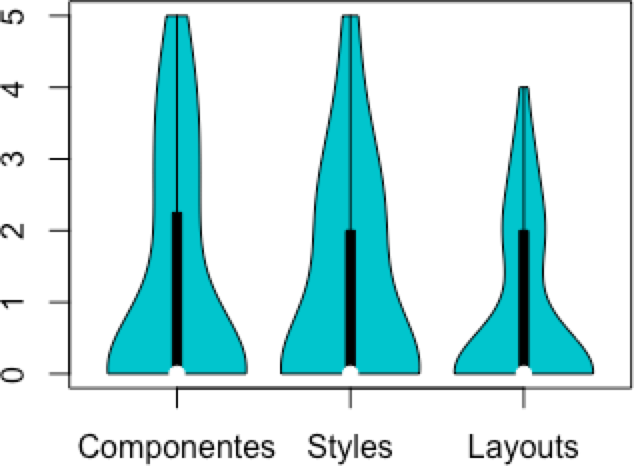
\includegraphics[width=.76\textwidth]{phase3-clean-violins-cutted.png}
  \caption{Componentes=\textit{Activities}, \textit{Fragments}, \textit{Adapters} ou \textit{Listeners} limpos. Styles=Recursos de \textit{Style} limpos. Layout=Recursos de \textit{Layout} limpos.}
  % \hspace*{-1cm}%
  \label{fig:clean-violins}
\end{subfigure}
\begin{subfigure}[t]{.48\textwidth}\centering
  % \hspace*{-1cm}%
  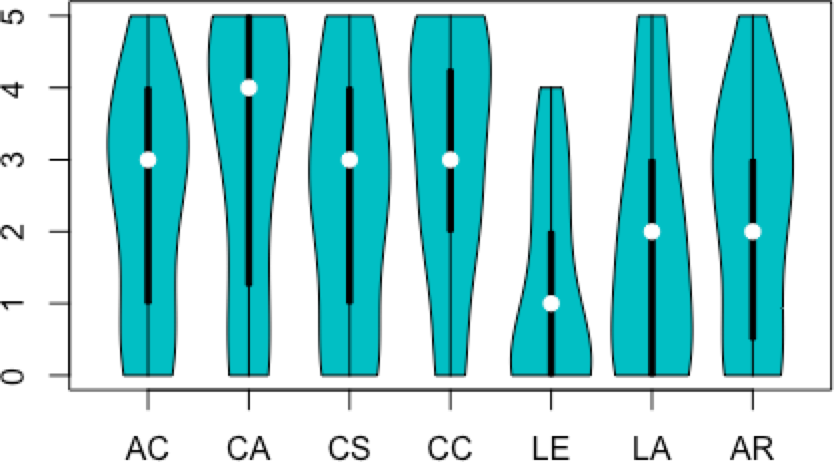
\includegraphics[width=1\textwidth]{phase3-smellys-violins2-cutted.png}
  \caption{AC=Adapter Complexo, CA=Componente de UI Acoplado, CS=Comportamento Suspeito, CC=Componente de UI Cérebro, LE=Longo Recurso de Estilo, LA=Layout Profundamente Aninhado, AR=Atributos de Estilo Repetidos.}
  % \hspace*{-1cm}%
  \label{fig:smellys-violins}
\end{subfigure}% 
\caption{Análise de severidade dos códigos limpos segmentados por grupos e dos códigos afetados pelos maus cheiros avaliados.}
\label{fig:}
% \vspace{-.5cm} 
\end{figure*}

A Figura \ref{fig:clean-violins} apresenta os gráficos violino sobre a percepção dos 3 grupos de códigos limpos: componentes Android, recursos de \textit{style} e recursos de \textit{layout}. Podemos observar que os 3 grupos de códigos apresentam mediana de severidade 0. Isso mostra que, como esperado, os códigos limpos, no geral, foram percebidos como limpos pelos desenvolvedores.

Muitos desenvolvedores, sem conhecer nosso catálogo de maus cheiros Android, foram capazes de identificar corretamente o mau cheiro, dando uma descrição do problema percebido muito próxima a definição do mau cheiro. Por exemplo, um deles ao se deparar com um \textsc{\small Adapter Complexo} relatou: \textit{``O método getView é muito longo, com muitos ifs. Dificultando testes, debug e entendimento. me parece que muitas variações de tela podem ser desenhadas nesse método.''}. Outro participante disse simplesmente: \textit{``getView faz muitas coisas. Isso é perigoso para manter.''}. 

Também o mau cheiro \textsc{\small Longo Recurso de Estilo}, foi corretamente identificado. Por exemplo, um dos participantes relatou: \textit{``Os temas e estilos poderiam ser separados em arquivos diferentes como por exemplo styles\_dialog.xml, styles\_text\_view.xml, etc inclusive em diretórios de recursos de acordo com nível de API do Android. Também poderia usar herança.''}. Outro participante disse apenas: \textit{``Muitos estilos no mesmo arquivo.''}. 

Outro participante ao se deparar com \textsc{\small Componente de UI Acoplado}, relatou: \textit{``Adapter está acoplado a MainActivity, uma vez que a recebe no construtor. O ideal seria abstrair quem está usando o Adapter para que ele possa ser usado por outras activities ou fragments.''}. Outros dois disseram simplesmente: \textit{``Cast direto à MainActivity.''} e \textit{``O DrawerAdapter está acoplado com a MainActivity.''}. Sobre o mau cheiro \textsc{\small Atributos de Estilo Repetidos}, um participante relatou: \textit{``1. Muitas dimensões repetidas que tem o mesmo propósito. Elas deveriam estar num lugar centralizado e nomeadas para facilidade de manutenção. 2. Mesma definição de estilo para várias text views. Deveria ser extraídas para styles para melhor manutenção...''}. Outro participante disse: \textit{``Muitos textViews com a mesma estilização, mas não se utiliza um arquivo de de styles para auxiliar.''}.

\begin{table}[!htb]
\centering
\renewcommand*{\arraystretch}{1}
\footnotesize
\caption{Dados estatísticos sobre a percepção negativa por desenvolvedores sobre os maus cheiros avaliados no experimento de código (S$_3$).} 
\begin{tabular}{@{}p{7cm}clcc@{}}
\toprule
\textbf{Mau Cheiro} & \multicolumn{1}{c}{\textbf{Valor de p ($\alpha$)}} & \multicolumn{1}{c}{\textbf{Delta de Cliff (\textit{d})}} & \textbf{Mediana} & \textbf{Q3} \\
\toprule
\textsc{\small Componente de UI Acoplado}       &  1,13e-04  &    0,52 (grande) & 4,00         & 5,00 \\
\textsc{\small Comportamento Suspeito}          &  1,37e-03  &    0,38 (médio)  & 3,00         & 4,00 \\
\textsc{\small Componente de UI Cérebro}        &  4,58e-06  &    0,55 (grande) & 3,00         & 4,25 \\
\textsc{\small Adapter Complexo}                &  1,11e-03  &    0,40 (médio)  & 3,00         & 4,00 \\
\textsc{\small Longo Recurso de Estilo}         &  7,61e-01  &    0,05 (insignificante) & 1,00 & 2,00 \\
\textsc{\small Layout Profundamente Aninhado}   &  6,17e-03  &    0,35 (médio)  & 2,00         & 3,00 \\
\textsc{\small Atributos de Estilo Repetidos}   &  5,84e-04  &    0,44 (médio)  & 2,00         & 3,00 \\
\bottomrule
\end{tabular}
\label{tab:smells-avaliados}
\end{table}


Foi possível confirmar estatisticamente a percepção dos desenvolvedores em 6 dos 7 maus cheiros Android avaliados. A Tabela \ref{tab:smells-avaliados} apresenta os valor de $\alpha$ e \textit{d} para todos eles, bem como informações de mediana e Q3. Apesar de haver respostas que identificaram corretamente o mau cheiro \textsc{\small Longo Recurso de Estilo} e do gráfico violino apresentar uma leve diferença de severidade dos recursos afetados pelo mau cheiro, com mediana 1 (Q3 = 2), contra os recursos limpos, são necessários mais dados para validá-lo estatisticamente. \\

\begin{square}
  \small
  Nossos resultados mostram que os códigos afetados pelos maus cheiros propostos e avaliados são percebidos como problemáticos por desenvolvedores Android se comparados com códigos limpos (QP$_3$).
\end{square}

